% !TEX root = ../main.tex

\subsection{ATLAS Humanoid Robot}

The valid control mode changes (c.f. Fig. \ref{Fig:ControlModeTS}) define a transition system $(\mathcal{M}, \boldsymbol\rightarrow)$, where $\mathcal{M}$ is the set of states, each corresponding to one control mode, $m \in \mathcal{M}$, and $\boldsymbol\rightarrow$ is a set of valid control mode transitions (subset of $\mathcal{M} \times \mathcal{M}$).
In addition, we define $Adj(m) = \{ m^\prime \in \mathcal{M} \; | \; (m, m^\prime) \in \; \boldsymbol\rightarrow \}$ and also allow self-transitions, i.e., $m \in Adj(m), \; \forall m \in \mathcal{M}$.

\begin{figure}[t]
\centering
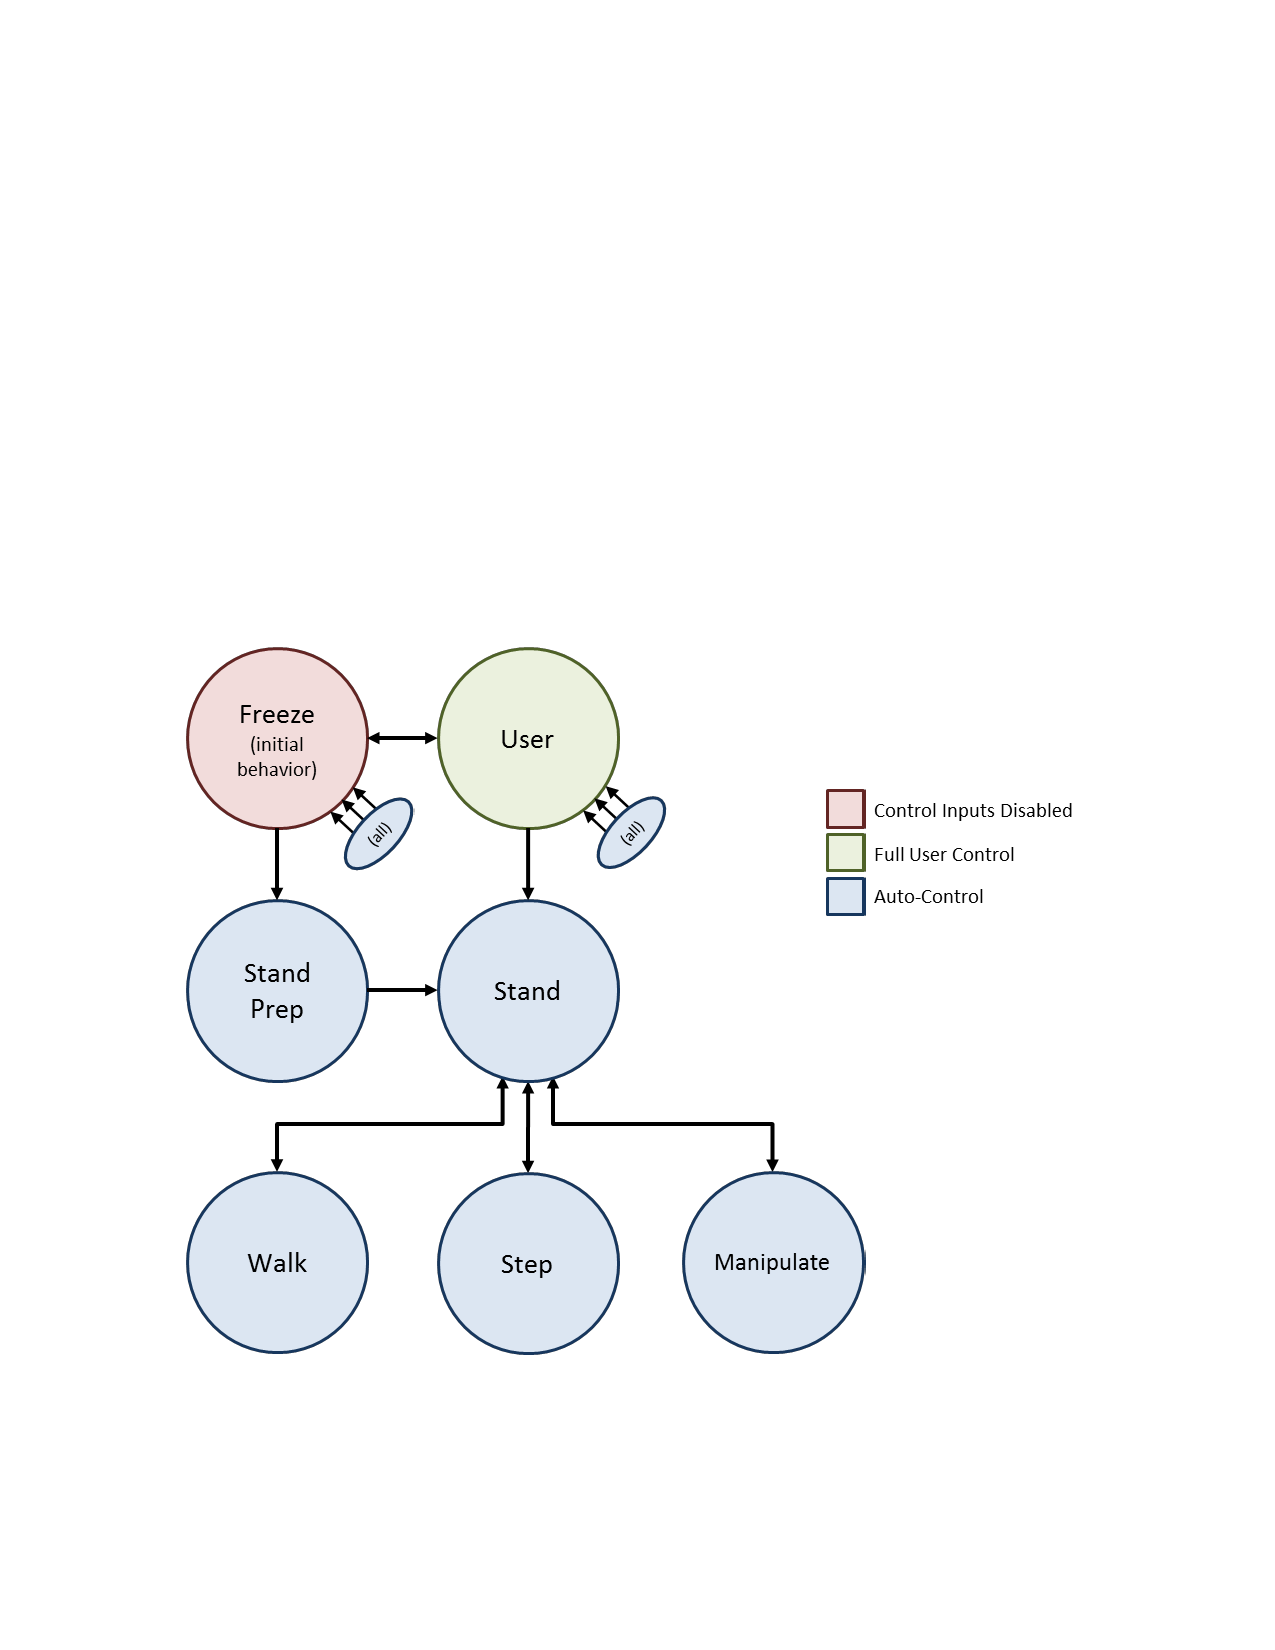
\includegraphics[width=0.95\columnwidth,clip]{./img/control_modes_ts.pdf}
\caption{
	\todo[inline, caption = {Create a simple control mode TS figure}]{Placeholder! Create two subfigures depicting a simple control mode TS and ATLAS doing something.}
}
\label{Fig:ControlModeTS}
%\vspace{-3 pt}
\end{figure}

\subsection{Team ViGIR's Approach to High-level Control}

\ldots

\subsection{Linear Temporal Logic and Reactive LTL Synthesis}

\ldots